
\documentclass[runningheads,a4paper]{llncs}

\usepackage{amssymb}
\setcounter{tocdepth}{3}
\usepackage{graphicx}
\usepackage{epstopdf}
\usepackage{float}
\usepackage{url}
\urldef{\mailsa}\path|{alfred.hofmann, ursula.barth, ingrid.haas, frank.holzwarth,|
\urldef{\mailsb}\path|anna.kramer, leonie.kunz, christine.reiss, nicole.sator,|
\urldef{\mailsc}\path|erika.siebert-cole, peter.strasser, lncs}@springer.com|
\newcommand{\keywords}[1]{\par\addvspace\baselineskip
\noindent\keywordname\enspace\ignorespaces#1}
\begin{document}
\author{}
\institute{}
\maketitle
%\vspace{-1cm}
% Please write your project tile in here
\section{Introduction}


\section{Applications for Identity-Based Encryption}
In this section, we show several applications of IBE
\subsection{Revocation of Public Keys}
Public key certificates are valid, an IBE system key expiration can be done by having Alice encrypt e-mail sent to Bob using the public key: “bob@company.com k current-year”.In this way, Bob can only use his private key within the time limit.This approach makes key revocation very simple. And Alice doesn't need to communicate with any third-party certificate directories to get Bob's daily public key.In addition, it can be used to manage user credentials, because Alice allows Bob to read messages within a specified date.
\subsection{Delegation of Decryption Keys}
Here are two examples to illustrate this function. Among them, Bob plays PKG, and Alice wants Bob to send email.\\
Delegation to a laptop\\
Suppose Alice wants Bob to send the message and uses the current date as the encryption key.Bob plans to travel for 7 days. When using IBE system, Bob can simply install seven private keys corresponding to the seven days of travel on his laptop.If the notebook is stolen in this area, only the private key of these seven days will be disclosed. The master key is not compromised.\\
Delegation of duties\\
Suppose Alice encrypts mail to Bob using the subject line as the IBE encryption key. Bob can decrypt mail using his master-key.Now, let's say Bob has several assistants, each responsible for a different task.Bob provides each assistant with a private key according to their duties.Each assistant can then decrypt messages for its subject line within its scope of responsibility, but not for other assistants.So IBE can simplify the management of a large number of public key security system.
\section{definition}
An identity-based encryption scheme E is specified by four randomized algorithms: Setup, Extract, Encrypt, Decrypt.\\
Setup:takes a security parameter k and returns params (system parameters) and master-key. \\
Extract:takes as input params, master-key, and an arbitrary ID$\in \{ 0,1 \}^*$,and returns a private key d.\\
Encrypt:takes as input params, ID, and $ m\in M$. It returns a ciphertext $c \in C$.
Decrypt:takes as input params, $c \in C$, and a private key d. It return $m \in M$.
$\forall m \in M$.: Decrypt(params, C, d) = m where c = Encrypt(params, ID, m).\\
IBE semantic security\\
definition 2.1. We say that the IBE system E is semantically secure against an adaptive chosen ciphertext attack if for any polynomial time IND-ID-CCA adversary A the function AdvE,A(k) is negligible.As shorthand, we say that E is IND-ID-CCA secure.\\
Initialization:Challenger generates system $\varepsilon$, and adversary a obtains the public key of the system.\\
Training: the enemy makes decryption inquiry to the Challenger (multiple times), that is, takes the ciphertext c to the challenger, the Challenger decrypts the panic, and gives the plaintext to the enemy. \\
Challenge: the opponent outputs two messages m0 and m1 with the same length, and then receives mb ciphertext from the challenger, where the random value b$\in \{ 0,1 \}$.\\
Guess: the opponent outputs b’, if b’ = b, then a succeeds.
\begin{figure}[H]
		\centering %图片居中
		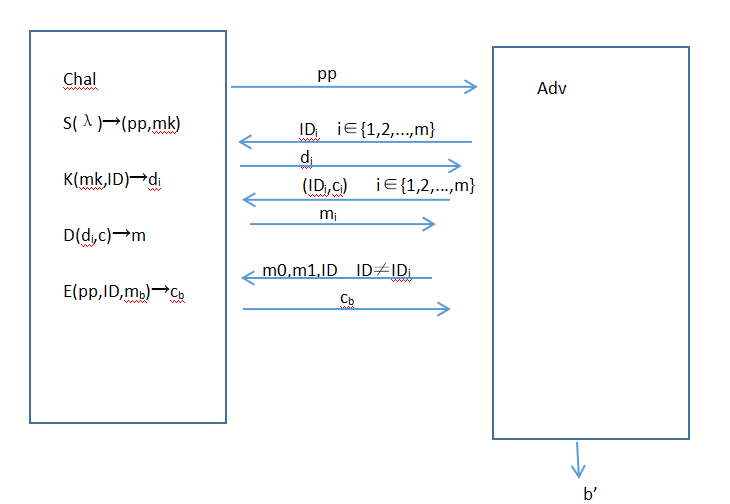
\includegraphics[width=0.8\textwidth]{./figure/CCA} %插入图片,[]中设置图片大小,{}中是图片文件名
		\caption{CCA} %最终文档中希望显示的图片标题
		\label{e} %用于文内引用的标签

\end{figure} 
Definition 2.2. We say that the IBE system E is semantically secure if for any polynomial time IND-ID-CPA adversary A the function AdvE,A(k) is negligible. As shorthand, we say that E is IND-ID-CPA secure.\\
Initialization:Challenger generates system $\varepsilon$, and adversary a obtains the public key of the system.\\
Challenge: the opponent outputs two messages m0 and m1 with the same length, and then receives mb ciphertext from the challenger, where the random value b$\in \{ 0,1 \}$.\\
Guess: the opponent outputs b’, if b’ = b, then a succeeds.
\begin{figure}[H]
		\centering %图片居中
		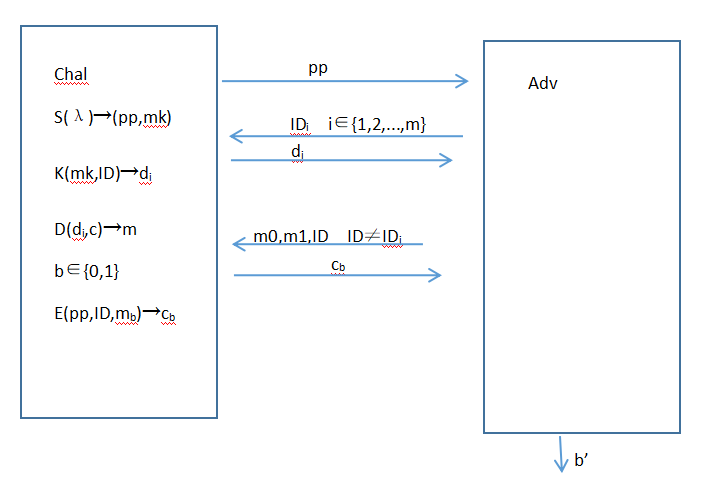
\includegraphics[width=0.8\textwidth]{./figure/CPA} %插入图片,[]中设置图片大小,{}中是图片文件名
		\caption{CPA} %最终文档中希望显示的图片标题
		\label{a} %用于文内引用的标签

\end{figure}
\section{Bilinear maps and the Bilinear Diffie-Hellman Assumption}
Let $ \mathbb{G}_{1}$ and $ \mathbb{G}_{2}$  be two groups of order q for some large prime q. Our IBE system makes use of a bilinear
map$\hat{e}: \mathbb{G}_{1} \times \mathbb{G}_{1} \rightarrow \mathbb{G}_{2}$ between these two groups. The map must satisfy the following properties:\\
1. Bilinear: We say that a map $\hat{e}: \mathbb{G}_{1} \times \mathbb{G}_{1} \rightarrow \mathbb{G}_{2}$is bilinear if $\hat{e}(a P, b Q)=\hat{e}(P, Q)^{a b}$ for all P, Q $\in \mathbb{G}_{1} $ and all a, b$\in \mathbb{Z} $.\\
2. Non-degenerate: The map does not send all pairs in $ \mathbb{G}_{1} X \mathbb{G}_{2}$  to the identity in$ \mathbb{G}_{2} $. Observe that since $ \mathbb{G}_{1},\mathbb{G}_{2} $ are groups of prime order this implies that if P is a generator of $\mathbb{G}_{1} $ then $\hat{e}(P, P)$ is a generator of $\mathbb{G}_{2} $.\\
3. Computable: There is an efficient algorithm to compute$\hat{e}(P, Q)$ for any P, Q $\in \mathbb{G}_{1} $ .\\
Decision Diffie-Hellman is Easy: The Decision Diffie-Hellman problem (DDH)  in $\mathbb{G}_{1} $ is to distinguish between the distributions $\langle P, a P, b P, a b P\rangle$ and $\langle P, a P, b P, c P\rangle$ where a, b, c are random
in $\mathbb{Z}_{q}^{*}$ and P is random in $\mathbb{G}_{1}^{*}$. Joux and Nguyen  point out that DDH in $\mathbb{G}_{1} $ is easy. To see
this, observe that given P, aP, bP, cP $\in \mathbb{G}_{1}^{*}$ we have\\$c=a b \bmod q \quad \Longleftrightarrow \quad \hat{e}(P, c P)=\hat{e}(a P, b P)$
\section{IBE}



\subsection{The Bilinear Diffie-Hellman(BDH) Assumption}

The security of Identity-Based Encryption(IBE) is based on the Bilinear Diffie-Hellman(BDH) Problem.


Let $\mathbb{G}_{1}, \mathbb{G}_{2}$ be two groups of prime order q. Let $\hat{e}: \mathbb{G}_{1} \times \mathbb{G}_{1} \rightarrow \mathbb{G}_{2}$ be an admissible bilinear map and let P be a generator of $\mathbb{G}_{1}$. The BDH problem in $\left\langle\mathbb{G}_{1}, \mathbb{G}_{2}, \hat{e}\right\rangle$ is as follows: Given $\langle P, a P, b P, c P\rangle$ for some $a, b, c \in \mathbb{Z}_{q}^{*}$ compute $W=\hat{e}(P, P)^{a b c} \in \mathbb{G}_{2}$. An algorithm A has advantage $\epsilon$ in solving BDH in $\left\langle\mathbb{G}_{1}, \mathbb{G}_{2}, \hat{e}\right\rangle$ if\\
             \centerline{${Pr}\left[\mathcal{A}(P, a P, b P, c P)=\hat{e}(P, P)^{a b c}\right] \geq \epsilon$}
The BDH hypothesis can be described as: \\
There is no probabilistic polynomial time algorithm has a nonnegligible advantage in solving BDH problems.
\subsection{BasicIdent}

BasicIdent is the basic IBE scheme. How it works is shown in the figure below ( BasicIdent Model). TA is trust authority and can be viewed as PKG. There are two hashes here, H1 for the hash ID, which is Alice's mailbox number. H2 is the result of a hash bilinear pair. This article uses the RO model, which simulates these two hashes.

\begin{figure}[H]
\centering
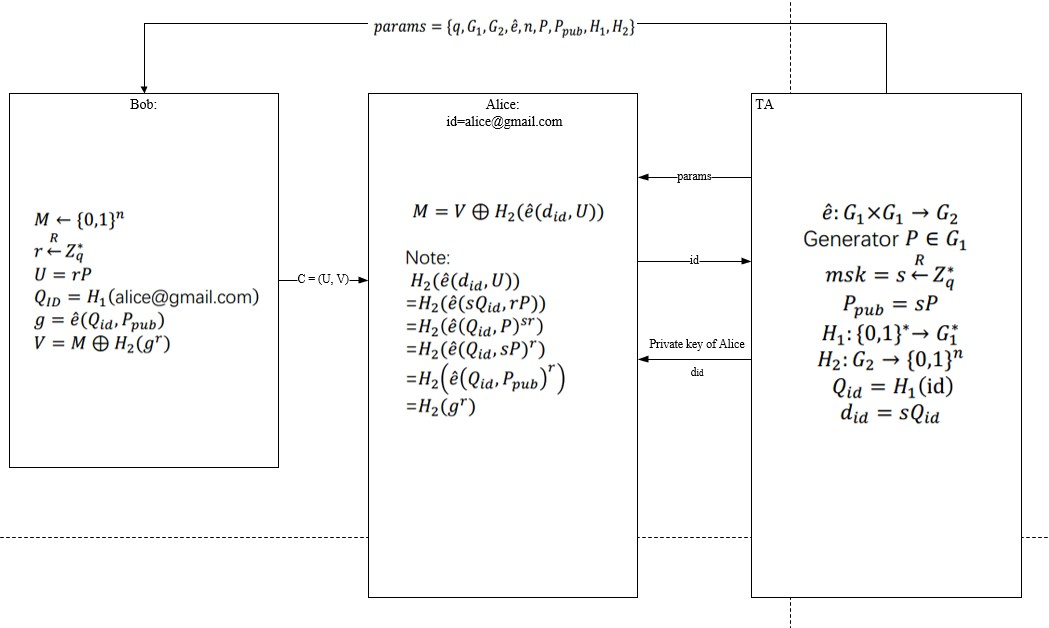
\includegraphics[width=10cm, height=7cm]{basicibe.JPG}
\caption{BasicIdent Model}
\end{figure}

The idea of specification proof is to first convert the above basic ident IBE scheme to a basic pub public key scheme. A relationship between these two advs is negligible. Then, the basicpub public key scheme can be reduced to BDH assumption. The following basicpub is the public key scheme after the specification. There is only one H2. The public key scheme does not need the previous ID, so it is useful to H1.

\begin{figure}[H]
\centering
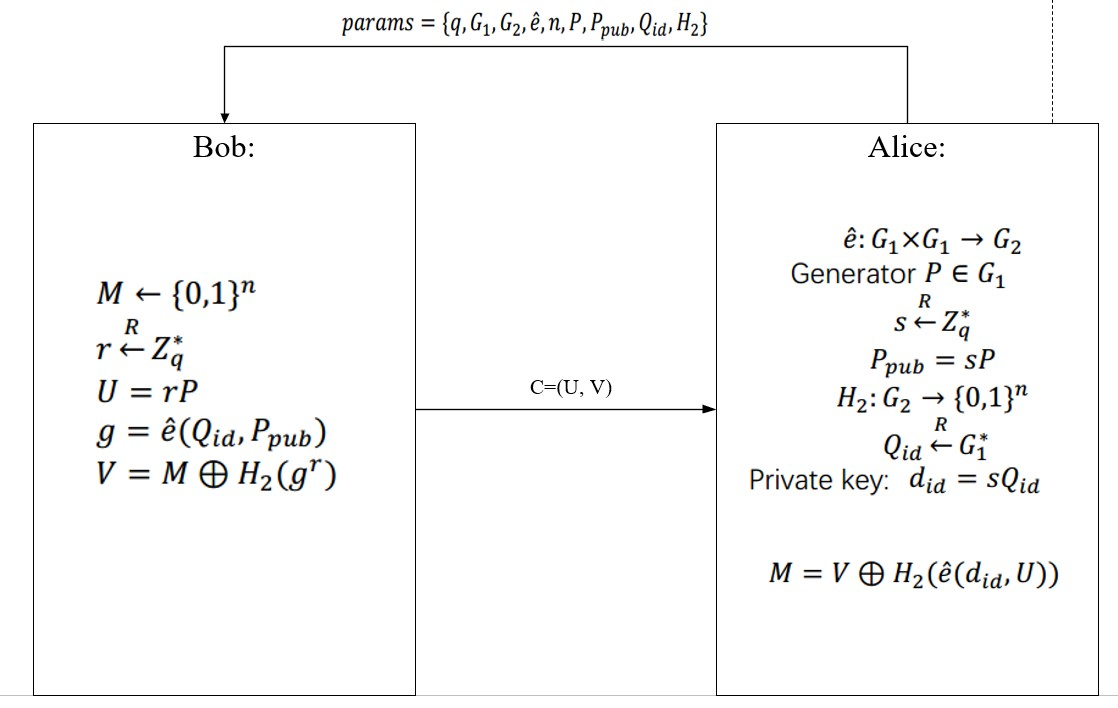
\includegraphics[width=10cm, height=7cm]{basicpub.JPG}
\caption{BasicPub Model}
\end{figure}

\subsection{Relaxing the hashing requirements}
IBE system uses a hash function $H_1:\{0,1\}^*\rightarrow\mathbb{G}_1^*$. Building such hash functions can be difficult. In order to relax the requirement of hashing. So an intermediate set $A$ is introduced. The scheme substitute hashing directly onto $\mathbb{G}_1^*$ into hashing onto $A\subseteq\{0,1\}^*$, and then map A onto $\mathbb{G}_1^*$ through a deterministic encoding function. 
The encoding function $L:A\rightarrow\mathbb{G}_1^*$ is admissible if it satisfies the following properties:
\begin{enumerate}
	\item Computable: An efficient deterministic algorithm to compute L(x) for any $x\in A$.
	\item $l$-to-1: $|L^{-1}(y)|=l$ for all $y\in \mathbb{G}_1^*$.
	\item Samplable: $\mathcal{L}_S(y)$ is a uniform random element in $L^{-1}(y)$
\end{enumerate}
The modification to FullIdent is to obtain and IND-ID-CCA secure IBE system. The $H_1$ is replaced by a hash function into some set $A$. It can be proved that the modified FullIdent is a chosen ciphertext secure IBE.
 
\section{A concrete IBE system using the Weil pairing}
The article then use FullIdent to describe IBE system based on the Weil pairing. 

The Weil pairing has some properties:
\begin{enumerate}
	\item Bilinear: For all $P,Q\in \mathbb{G}_1$ and for all $a,b\in \mathbb{Z}$ it satisfy $\hat{e}(a P, b Q)=\hat{e}(P, Q)^{a b}$.
	\item Non-degenerate: If $P$ is a generator of $\mathbb{G}_1$ then $\hat{e}(P, P) \in \mathbb{F}_{p^{2}}^{*}$ is a generator of $\mathbb{G}_2^*$
	\item Computable: Given $P, Q \in \mathbb{G}_{1}$ an efficient algorithm to compute $\hat{e}(P, Q) \in \mathbb{G}_{2}$ exists.
\end{enumerate}
Computational Diffie-Hellman problem (CDH) is hard in the group $\mathbb{G}_1$ and Decisional Diffie-Hellman problem (DDH) is easy in $\mathbb{G}_1$. Later, the author introduced the BDH Parameter Generator into discussion and draw the conclusion that one should not use this BDH parameter generator with primes p that are less than 512-bits long.
\subsection{An admissible encoding function: MapToPoint}
As the IBE system uses a hash function $H_1:\{0,1\}^*\rightarrow\mathbb{G}_1^*$. The author presentated an admissible encoding function $MapToPoint$.
the MapToPoint work as follows:
\begin{enumerate}
	\item Compute $x_{0}=\left(y_{0}^{2}-1\right)^{1 / 3}=\left(y_{0}^{2}-1\right)^{(2 p-1) / 3} \in \mathbb{F}_{p}$
	\item Let $Q=\left(x_{0}, y_{0}\right) \in E\left(\mathbb{F}_{p}\right)$ and set $Q_{\mathrm{lo}}=\ell Q \in \mathbb{G}_{1}$
	\item Output $MapToPoint(y_0)=Q_{ID}$ 
\end{enumerate}
The admissibility of $MapToPoint$ is proved.

\section{Extensions and Observation}
The author presented some extensions. The system based on some other curves such as Tate pairings are discussed with the conclusion that encryption and decryption in FullIdent can be made faster by using the Tate pairing on elliptic curves. The application of IBE in an e-mail system storing the CA's private key in PKG is also mentioned. The PKG's master-key can be generated in a distributed fashion. In addition, the performance of the IBE system can be optimized by working in a small subgroup of the curve. 

\section{Escrow EIGamal encryption}
The escrow ability to EIGamal encryption system can be obtained through the Weil pairing. It gives the algorithm under the setup of BDH parameter generator $\mathbb{G}$ and a security parameter $k \in \mathbb{Z}^+$. The system is semantic secure when BDH is hard for groups generated by $\mathcal{G}$.

\section{Conclusion}
The article introduced the fully functional IBE system. The system is built under in random oracle model with the assumption BDH, which is a natural analogue of the computational Diffie-Hellman problem. The article applied one transformation method from Fujisaki-Okamoto to convert basic BasicIdent scheme into ciphertext secure IBE system in random oracle model as FullIdent. In addition, a concrete IBE system using the Weil pairing and extensions and observations of the scheme are also discussed. To build chosen ciphertext secure identity based systems is currently an open problem.

\section{appendix}
Wangzhihui Mei has surveyed the basic IBE scheme BasicIdent and the method of relaxing the hashing requirements of FullIdent as well as the example IBE system based on weil pairing. Then Mei watched some extension usage of the introduced IBE system and escrow EIGamal encryption system.
\end{document}